\documentclass[twocolumn]{article}
\usepackage{graphicx}
\usepackage{amsmath}
\usepackage{siunitx}
\usepackage{fancyhdr} 
\usepackage{fancybox}
\usepackage{float}
\usepackage{listings}
\usepackage[colorlinks=true,linkcolor=black]{hyperref}
%\usepackage[labelformat=empty]{caption}
\usepackage[margin=1.0in]{geometry}
\usepackage[section]{placeins}
\pagestyle{fancy}

%redefines subsections with letters instesad of numbers
\renewcommand{\thesubsection}{\thesection.\alph{subsection}}

% Center Image Command
\newcommand{\centerimage}[3]{
\begin{figure}[ht!]  
\begin{center} #1
\caption{#2}
\label{#3}
\end{center}
\end{figure}}

\newcommand{\tstamp}{\today}   
%\renewcommand{\chaptermark}[1]{\markboth{#1}{}}
\renewcommand{\sectionmark}[1]{\markright{#1}}
\lhead[\fancyplain{}{\thepage}]         {\fancyplain{}{Andy Goetz \& Kevin Riedl}}
\chead[\fancyplain{}{}]                 {\fancyplain{}{}}
\rhead[\fancyplain{}{\rightmark}]       {\fancyplain{}{ECE 486 Branch Target Buffer Predictor \& Alpha Predictor}}
\lfoot[\fancyplain{}{}]                 {\fancyplain{\tstamp}{\tstamp}}
\cfoot[\fancyplain{\thepage}{}]         {\fancyplain{}{}}
\rfoot[\fancyplain{\tstamp} {\tstamp}]  {\fancyplain{}{\thepage}}

\author{\LARGE Andy Goetz \& Kevin Riedl}
\date{\today}
\title{\Huge \textbf{ECE 486 Branch Target Buffer \& Alpha Predictor} \\ \rule{\linewidth}{0.5mm}}

\begin{document}
\maketitle
\section{Abstract}
\section{Acknowledgements}

The authors would like to thank Tyler Tricker, Bradon Kanyid, and Eric
Krause for the many hours of fruitful discussions. Additionally, they
would like to thank Beth Krause for the delicious cookies provided.

\section{Background Information}
The purpose of this project was to develop a branch predictor for an
unknown ISA. We were required to copy the branch predictor used in the
Alpha 21264 processor. We were then required to design a branch target
predictor, with the requirement that it use only 8 kilobytes of
state. This branch predictor was then tested against an array of 20
test traces, in order to determine its performance. 


\section{Branch Predictor}
The branch predictor used in this project was modeled after
The one described in R. E. Kessler's paper on the Alpha 
21264 processor. 

Since the Alpha paper does not specify a few details about how the predictor
works, liberties were taken in determining the best prediction values. 

\centerimage{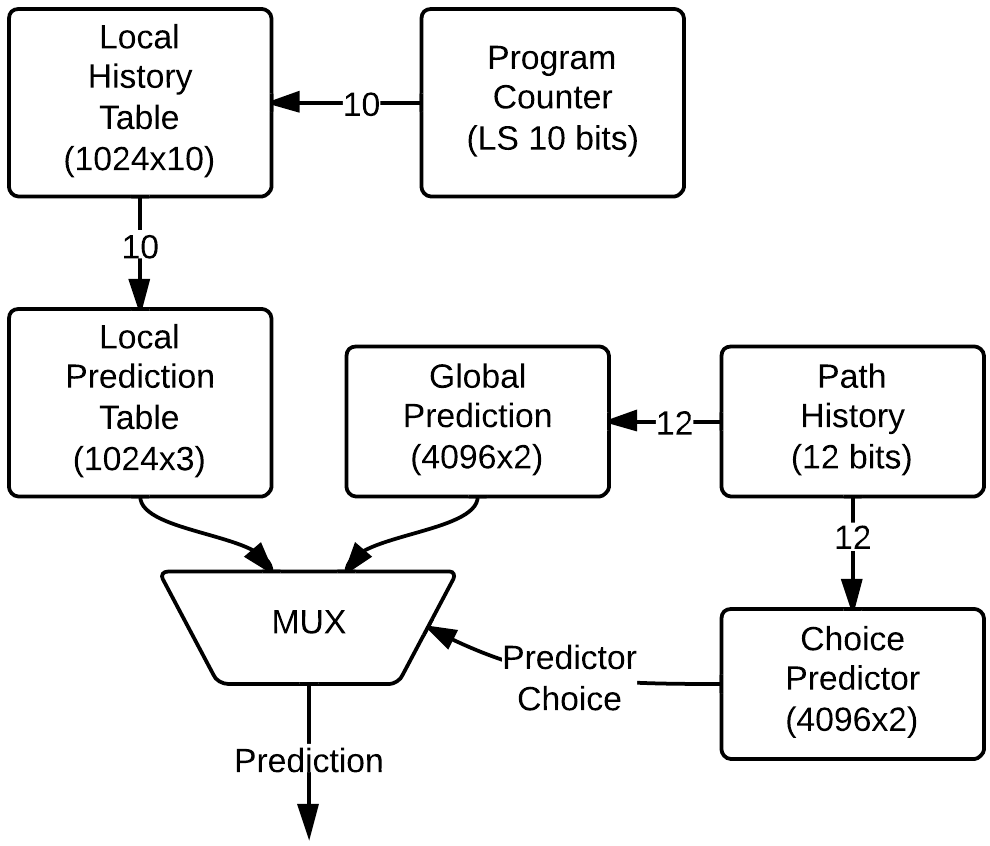
\includegraphics[width=\columnwidth]{AlphaPredictor.png}}{Alpha Predictor}{Alpha}
\subsection{Initialized Values}

The Alpha paper did not specify which values to initialize the tables with.
Fortunately, once many branches have occurred, the initial values do not matter
when looking at a system which processes billions of branches between power downs.
For the relatively small trace data set used in these simulations however,
the initialization values were important for determining more accurate branch prediction.
For example, Changing the Global Predictor from weakly taken to weakly not taken changes 
the average $\frac{\#\,of\,mispredicts}{1000\,\text{instructions}}$ from $14.10950$ to $14.07025$
respectively, which is a significant performance improvement.
 
\subsection{Unconditional Branch Inclusion in the Path History}

The Path History is important in determining which predictor to use
in the case of the Choice Predictor and it is important in determining
which saturating counter to use in the case of the Global Predictor.
The Alpha predictor described in the paper did not specify whether or not
unconditional branches are included in the Path History (i.e. jumps), but
could change the results of these predictors significantly. Testing both 
possibilities determined that the exclusion of the unconditional branches 
yielded more accurate branch prediction, thus this implementation is using
a Path History that ignores uncoditonal branches.

\section{Branch Target Predictor} 

In order to be truly successful, a branch predictor must be carefully
tuned to its target workload. The fact that the set of all traces our
branch predictor would be tested against was known ahead of time
presented us with an unbridled opportunity for "benchmarketing",
however, we still needed to gather information about the traces, in
order to design an effective branch target predictor. 

\subsection{Displacement Cache}
Figure \ref{ddelta} shows the ECDF (Empirical Cumulative 
Distribution Function) first four benchmarks. As can be 
seen from this graph, most branches have destinations that 
are relatively close to the source program counter. From 
this, it follows that a branch target buffer that only 
stores the displacement to branch destination could achieve 
close to the same performance as a cache with direct-mapped 
branch destinations, while consuming less memory. 

\centerimage{\includegraphics[width=\columnwidth]{ecdf-serv-delta.pdf}}{CDF
  of Branch Displacement Size}{ddelta}


\begin{table}\begin{center}\begin{tabular}{ll}

Entry Size (bits) & Storeable Branches \\
\hline
4 & 3.5\% \\
8 & 51.9\% \\
12 & 66.3\% \\
16 & 81.8\% \\
24 & 95.1\% 
\end{tabular}\end{center}
\caption{Displacement Cache Capacity}
\label{dtable}
\end{table}

Table \ref{dtable} shows percentage of the branch targets that could
fit in a buffer entry of 4, 8, 12, 16, and 24 bits. As can be seen by
the table, while a larger displacement field can store a greater
percent of the branch targets, even a 24 bit entry can only hold 95\%
of branch targets. However, an 8 bit entry can store over half of the
possible branch targets. This suggests a hybrid approach: use two
caches, one that only holds branches that can fit in a small
displacement, and another that stores branch targets that are too
large for the displacement field. This allows us to get performance
that is close to that of a larger cache, while using less space. A 64
entry by 10 way cache uses 77056 bits, while a combination of a 8 way
main cache and 2 way displacement cache only uses 30720 bits, and
achieves similar performance.

\subsection{Return Address Stack}
Another way that we sought to increase branch target performance was
by using a Return Address Stack (RAS). Figure \ref{btype} shows the
distribution of branch types in four of the benchmark programs. As can
be seen from the graph, subroutine returns make up a not insubstantial
part of each trace file, especially the server benchmark. 

\centerimage{\includegraphics[width=\columnwidth]{btype.pdf}}{Branch Type Distribution}{btype}


\subsection{Target Predictor Implementation}

The branch target predictor used in the simulator can be seen in
figure \ref{btbshape}. It is based on a hierarchy of two separate
caches, combined with a return address stack. A small displacement
cache (64 entries by 2 ways) holds entries whose target address is
less than 128 bytes from the program counter. If a target address has
a displacement that is too large to fit in this cache, or an address
is evicted from the displacement cache, it is placed in another,
larger cache that contains direct-mapped addresses. This larger cache
is organized as 64 entries by 8 ways.

\centerimage{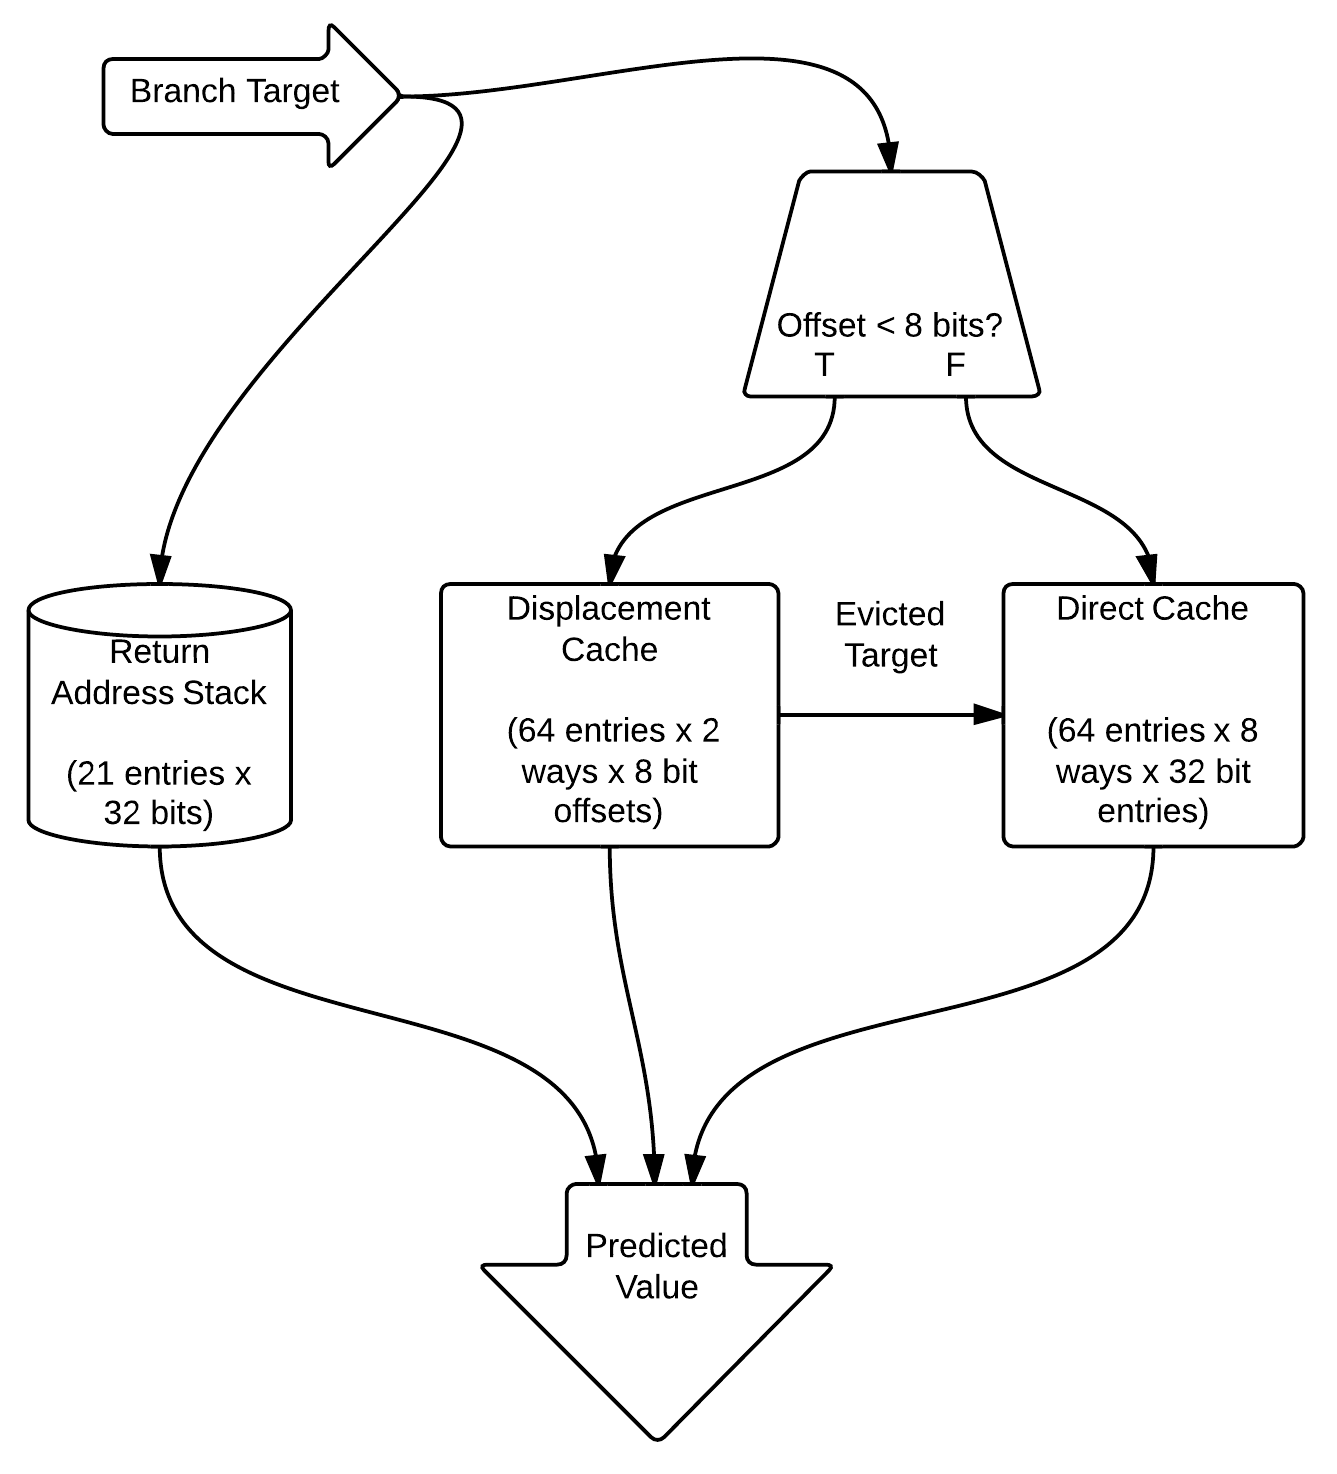
\includegraphics[width=\columnwidth]{BTB.png}}{Branch
  Target Predictor}{btbshape}

The branch target predictor also contains a return address stack. This
stack stores the return address of the last 21 calls. This allows
return addresses to be predicted, regardless of whether or not they
are in the cache. In addition to storing return addresses in the RAS,
return addresses are also placed in the displacement and direct
caches.

\section{Testing Methodology}

In order to determine the optimal branch predictor design, a generic
predictor framework was designed that used environment variables to
determine the cache hierarchy used by the branch target predictor.
The tunable parameters can be seen in table \ref{envars}. 

\begin{table}
\begin{center}\begin{tabular}{p{.35\columnwidth}p{.5\columnwidth}}
Variable Name & Description \\
\hline
\texttt{BTB\_MAIN\_SIZE} & Index bits of direct cache \\
\texttt{BTB\_MAIN\_WAYS} & Number of ways of direct cache \\
\texttt{BTB\_DISP\_ENTRIES} & Size of entry for displacement cache \\
\texttt{BTB\_DISP\_SIZE} & Index bits of displacement cache \\
\texttt{BTB\_DISP\_WAYS} & Number of ways of displacement cache \\
\texttt{BTB\_WAY\_ALGO} & Way Eviction Policy (LRU or Round Robin) \\
\texttt{BTB\_FUNC\_CAP} & Number of entries in RAS
\end{tabular}\end{center}
\caption{BTB Tunable Parameters}
\label{envars}
\end{table}

In addition, a replacement predictor framework was written using
plaintext tracefiles, allowing for much faster traces, as well as more
detailed predictor statistics. These statistics included a breakdown of
the percentage of misses that were caused by function calls,
conditional branches, and indirect branches, among other values. 


\centerimage{\includegraphics[width=\columnwidth]{random.pdf}}{Performance
  of Random Sized BTB Caches}{bgraph}
%Oracle predictor and BTB variables
%Table comparing Faust results to our results for Alpha
\section{Results}
%Table with all prediction rates for all tests
\section{Conclusion}
\newpage
\onecolumn
\section{Predictor.cc}
\lstinputlisting{../predictor.cc}[language=C++, showstringspaces=false]
\end{document}

